\documentclass[a4paper]{article}

\usepackage[english]{babel}
\usepackage[utf8]{inputenc}
\usepackage{amsmath}
\usepackage{graphicx}
\usepackage[colorinlistoftodos]{todonotes}
\usepackage{natbib}
\usepackage{float}
\usepackage{blindtext}
\usepackage{authblk}
\title{\textbf{Dimension Reduction}\\ \large Linear Algebra Project Report, Dr.Ramin Javadi}
\author[1]{MohammadSadegh Akhoundzadeh\thanks{ms.akhondzadeh@gmail.com}}
\author[1]{Maryam Meghdadi\thanks{marmegh@gmail.com}}
\affil[1]{Department of Electrical and Computer Engineering, Isfahan University of Technology
}

%\subt {Linear Algebra Project Report, Dr.Ramin Djavadi}



\begin{document}
\maketitle

\begin{abstract}
In this report we give a review on some methods of dimension reduction. Given some input high-dimensional data, the goal of dimension reduction is to map them to a low-dimensional space such that certain properties of the initial data are preserved. Finally, we will compare discussed methods in some experiments.
\end{abstract}

\section{Introduction}
\label{sec:introduction}

In machine learning classification problems, there are often too many factors on the basis of which the final classification is done. These factors are basically variables called features. The higher the number of features, the harder it gets to visualize the training set and then work on it. Sometimes, most of these features are correlated, and hence redundant. This is where dimensionality reduction algorithms come into play. Dimensionality reduction is the process of reducing the number of random variables under consideration, by obtaining a set of principal variables. It can be divided into feature selection and feature extraction.
Some of the dimension reduction methods are based on linear transformation like PCA (Principal Component Analysis) and some of them are based on nonlinear techniques such as Isomap and Spectral Embedding.
\section{Theory}
\label{sec:theory}

\subsection{Linear Methods}

\subsubsection{PCA}
Principal component analysis(PCA) is a very popular technique for dimensionality reduction. Given a set of n-dimensional data, PCA algorithm aims to find d-dimensional data (d $<$ n) on a linear subspace. Such a reduced subspace
attempts to maintain most of the variability of the data. The linear subspace can be specified by d orthogonal vectors that form a new coordinate
system, called the 'principal components'. The goal is to find some vectors on a subspace which the variation of the data is maximal on it.\\
\textbf{Example:} In this example we projected a 3D data in a 2D subspace. Actually, we project the data on the plane of two eigenvectors U1 and U2.(Figure 1)\\

\begin{figure}
\centering
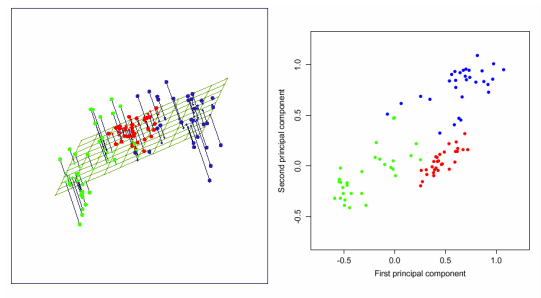
\includegraphics[width=1.1\textwidth]{pca.png}
\caption{\label{fig:pca}PCA applied to a 3D data set to reduce it to two dimensions}
\end{figure}

In order to capture as much of the variability as possible, let us choose the first principal component, denoted by $U_1$, to have maximum variance. Our data is n $\times$ t matrix X and our first eigenvector is a combination of X with $\omega$ coefficients such that $\omega$ = [$\omega_1 \ldots \omega_n$]. So we have:
\begin{equation}
U_1 = \omega^T X 
\end{equation}
\begin{equation}
\text{var}(U_1) = \text{var}(\omega^T X) = \omega^T S \omega
\end{equation}
where S is the n $\times$ n sample covariance matrix of X. 
To reach our goal we should maximize the variance we obtained in (2).
\begin{center}  
max  $\omega^T$S $\omega$ \space \space s.t. $\omega^T \omega$ = 1 
\end{center}
To do this, we use lagrange method and introduce a lagrange multiplier $\lambda$:
\begin{equation}
L(\omega, \lambda) = \omega^T S \omega - \lambda(\omega^T \omega - 1)
\end{equation}
By differentiating L with respect to $\omega$ we have:
\begin{equation}
S\omega = \lambda_1\omega
\end{equation}
This shows that the first principal component is given by the normalized eigenvector with the largest associated eigenvalue of the sample covariance matrix S. A similar argument can show that the d dominant eigenvectors of covariance matrix S determine the first d principal components. To obtain these eigenvectors we find singular value decomposition (SVD):
\begin{equation}
X = U \Sigma V^T
\end{equation}
where columns of U are eigenvectors of $XX^T$ (covariance matrix).
We define Y as our projected d-dimensional data (d $<$ n):
\begin{equation}
Y = U(:, 1:d)^T X \qquad or \qquad Y = U_d^T X
\end{equation}
Next step is to reconstruct the training data which is:
\begin{equation}
\hat{X} = U_d Y
\end{equation}
For a new test example x we compute $y = U^T x$ and then reconstruct it $\hat{x} = U y$ .
%In general, from (2) and (4) we have:
%\begin{equation}
%\omega^T S \omega = \omega^T \lambda \omega = \lambda
%\end{equation}
%and final variance is:
%\begin{equation}
%\sum_{i = 1}^{t} \text{var}(
%\end{equation}
% check n & t
[2]

\subsubsection{Dual PCA}
Dual PCA is similar to PCA but it's using a trick that make this method faster in the case that the number of features is bigger than the samples. The goal is to reduce dependence of our algorithm on n (the number of features). So instead of decomposition of $XX^T$, we decompose $X^TX$. Note that in the SVD factorization $U\Sigma V^T$, so $XV = U\Sigma$, where the eigenvectors in U corresponds to nonzero singular values in $\Sigma$. Thus, the following conversion between the top d eigenvectors can be derived:
\begin{equation}
U = XV\Sigma^{-1}
\end{equation}
Replacing all uses of U in PCA algorithm gives us Dual PCA algorithm. First we compute Y:
\begin{equation}
Y = U^TX = \Sigma V^T
\end{equation}
Then, reconstruct data:
\begin{equation}
\hat{X} = UY = U\Sigma V^T = XV\Sigma^{-1}\Sigma V^T = XVV^T
\end{equation}
Next, project out of sample point x:
\begin{equation}
y = U^T x = \Sigma^{-1} V^T X^T x 
\end{equation}
And finally reconstruct this sample point:
\begin{equation}
\hat{x} = U y = UU^T x = XV\Sigma^{-2} V^T X^T x 
\end{equation}

\subsubsection{Random Projection}
Again, if the number of samples is large, we can use a random method which guarantees that after projecting the points from the n-dimensional
space to K dimensional space using the randomly drawn matrix W, the distances between the high dimensional points is preserved in the lower dimensional projections up to some approximation factor. This matrix W is:

\[
W[i,j] = \left\{
				\begin{array}{ll}
				+\frac{1}{\sqrt{K}} \qquad \text{with probability 1/2}\\
                -\frac{1}{\sqrt{K}} \qquad \text{with probability 1/2}
				\end{array}
         \right \}
  \]      

\subsection{Nonlinear Methods}

\subsubsection{Isomap}
The euclidean distance of points on a linear space remains unchanged but on a submanifold (nonlinear space) this distance will change. This method is similar to MDS but we change euclidean distance to geodesic distance. The
geodesic distances represent the shortest paths along the curved surface of the manifold measured as if the surface were flat. This can be approximated by a sequence of short steps between neighboring sample points. Isomap then applies MDS to the geodesic rather than straight line distances to find a low-dimensional mapping that preserves these pairwise distances.
Steps of Isomap are:
\begin{enumerate}
\item Construct a k-nearest neighbor graph on n data points (connect each point to it's k-nearest neighbor.

\item Compute shortest path between all the points ($D^G$) as an estimation of geodesic distance, using Dijkstra's algorithm and Floyd-Warshall's algorithm.

\item Compute $k = -\frac{1}{2} H(D^G)^2 H$. find eigenvectors of k and call it V. then find the top p eigenvalues of k and form $\hat{\Lambda}$. The final solution is $Y = {\hat{\Lambda}}^\frac{1}{2} V^T$. Note that matrix H is a centering matrix and is equal to $H = I - \frac{1}{n}e e^T$, where e is a n $\times$ 1 vector of ones and $\hat{\Lambda}$ is a diagonal matrix which diagonal values are the top p eigenvalues of $X^T X$.

\end{enumerate}

\subsubsection{Laplacian Eigenmaps (Spectral Embedding)}
Given t points in n-dimensional space, the Laplacian eigenmaps Method (LEM)  starts by constructing a weighted graph with t nodes and a set of
edges connecting neighbouring points. The neighbourhood graph can be
constructed by finding the k nearest neighbours. For weighting the edges, we can use adjacency matrix, which elements are one for the nodes that are connected and zero for disconnected nodes. Another way is to use gaussian distance:
\begin{equation}
W_{ij} = e{^{-\frac{||x_i - x_j|| ^ 2}{\gamma}}}
\end{equation}
The embedding map is then provided by the following objective:
\begin{equation}
\min_{Y} \sum_{i = 1}^{t} \sum_{j = 1}^{t} (y_i - y_j)^2 W_{ij}
\end{equation}
subject to appropriate constraints. From spectral clustering we know that:
\begin{equation}
\sum_{i,j} (y_i - y_j)^2 W_{ij} = Y^T L Y 
\end{equation}
So From (14) and (15) we reach to:
\begin{equation}
\min_{Y} Tr(YLY^T)  
\end{equation}
\begin{center}
 \text{s.t.} $YY^T = I$\\
\end{center}
Where L is laplacian matrix which is $L = D - W$ and D is diagonal and equals to $D_{ii} = \sum_{j=1}^{t} W_{ij}$. From (13) and (15) we conclude that if $x_i$ and $x_j$ are far apart then $W_ij$ becomes small, so we don't care about $y_i$ and $y_j$. But if $x_i$ and $x_j$ are close, $W_ij$ becomes large, so $y_i$ and $y_j$ should be small and we reach to our goal.

\section{Experiment}
We start by generating three different data to compare the algorithms.
\subsection{Part1}

At first we create data in the shape of "hello"(figure 2). 
\begin{figure}[H]
\centering
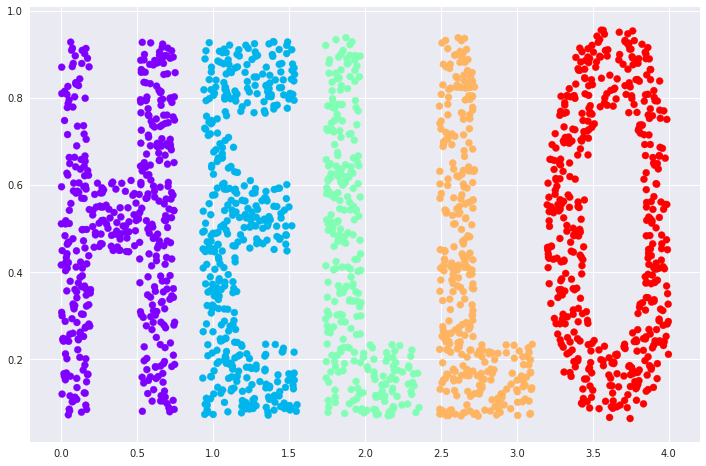
\includegraphics[scale = 0.33]{simple_hello.png}
\caption{\label{fig:simple_hello}hello-shaped data}
\end{figure}
Then for the first part of our experiments we use a linear function with a gaussian noise to add a new dimension to the data and make it 3D. (figure 3)
\begin{figure}[H]
\centering
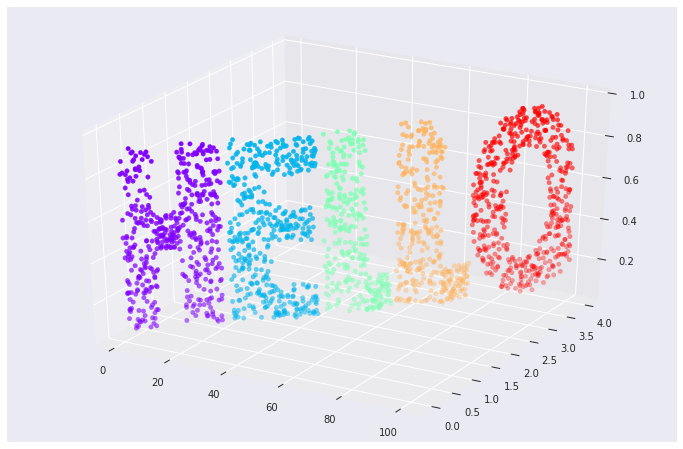
\includegraphics[scale = 0.33]{3_dhello_linear_gussian.png}
\caption{\label{fig:3_dhello_linear_gussian}3D hello-shaped data}
\end{figure}
\newpage
See the result of the the algorithms below:
\begin{figure}[H]
\centering
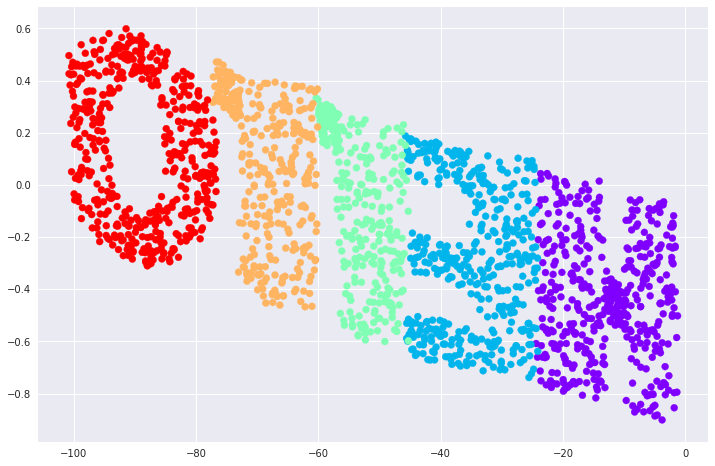
\includegraphics[scale = 0.32]{pca_part1.png}
\caption{\label{fig:pca_part1}PCA applied to 3D hello(figure 3) set to reduce it to two dimensions}
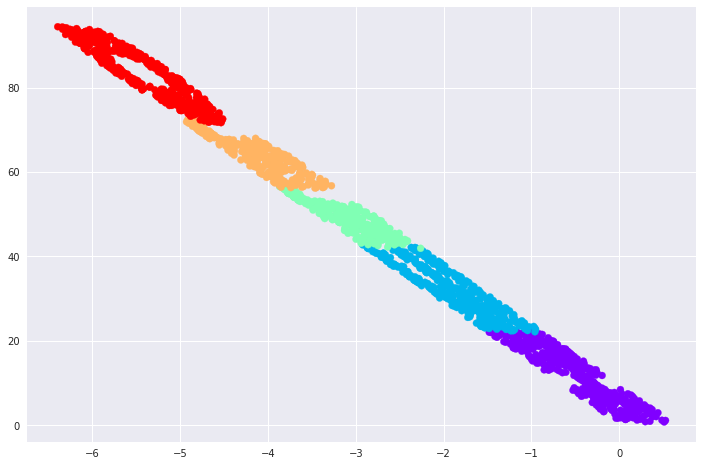
\includegraphics[scale = 0.32]{random_projection_part1.png}
\caption{\label{fig:random_projection_part1}Random Projection applied to 3D hello(figure 3) set to reduce it to two dimensions}

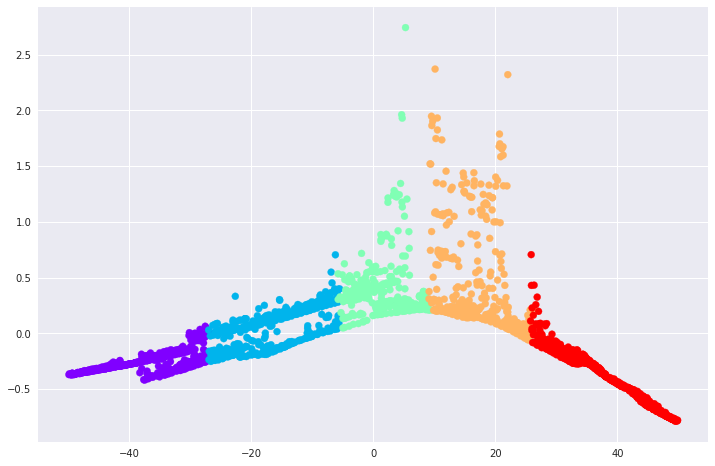
\includegraphics[scale = 0.32]{isomap_part1.png}
\caption{\label{fig:isomap_part1}Isomap applied to 3D hello(figure 3) set to reduce it to two dimensions}

\end{figure}

\begin{figure}[H]
\centering
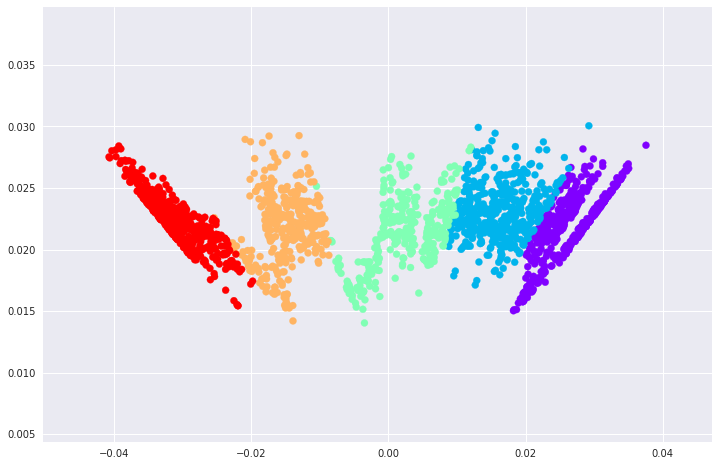
\includegraphics[scale = 0.32]{laplacian_part1.png}
\caption{\label{fig:laplacian_part1}Laplacian applied to 3D hello (figure 3) set to reduce it to two dimensions}
\end{figure}

%\begin{figure}
%\centering
%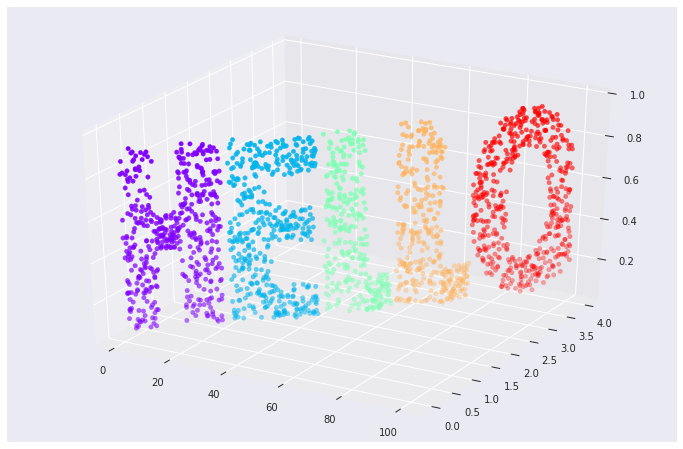
\includegraphics[scale = 0.4]{3_dhello_linear_gussian.png}
%\caption{\label{fig:3_dhello_linear_gussian}...}
%\end{figure}

\subsection{Part2}
In the next part instead of adding a new dimension to the data, we maked the “hello” data curved (figure 8)
\begin{figure}[H]
\centering
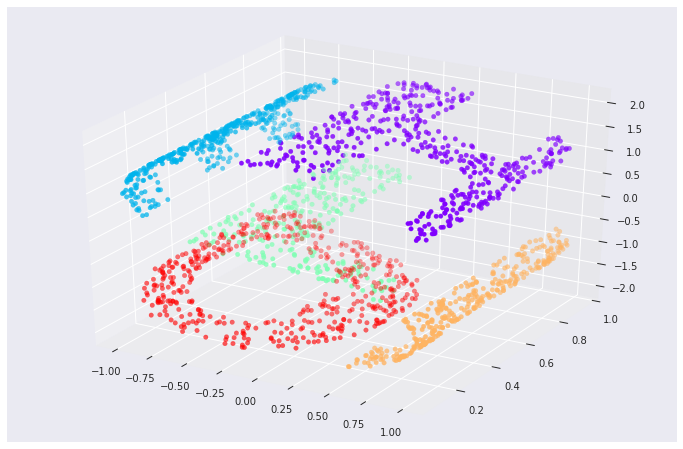
\includegraphics[scale = 0.32]{curved_hello.png}
\caption{\label{fig:curved_hello}curved hello}
\end{figure}
so now we have a manifold in the shape of “hello” in three dimensions and our goal is to reduce the dimension while preserving the certain properties of the data. 
\newpage 
See the result of the the algorithms below:
\begin{figure}[H]
\centering
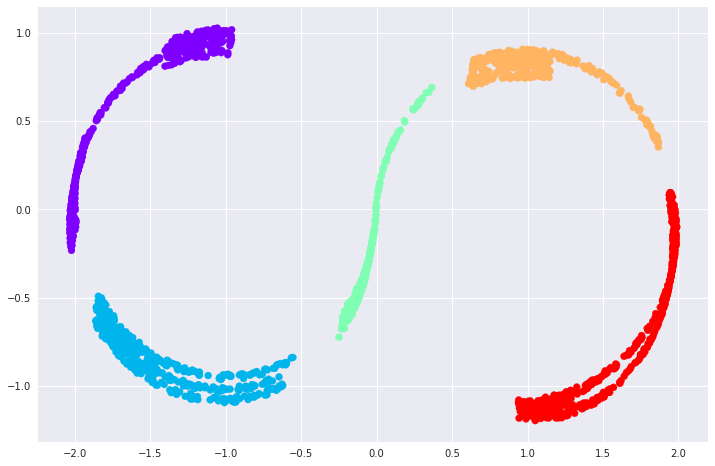
\includegraphics[scale = 0.32]{pca_part2.png}
\caption{\label{fig:pca_part2}PCA applied to curved hello (figure 8) set to reduce it to two dimensions}
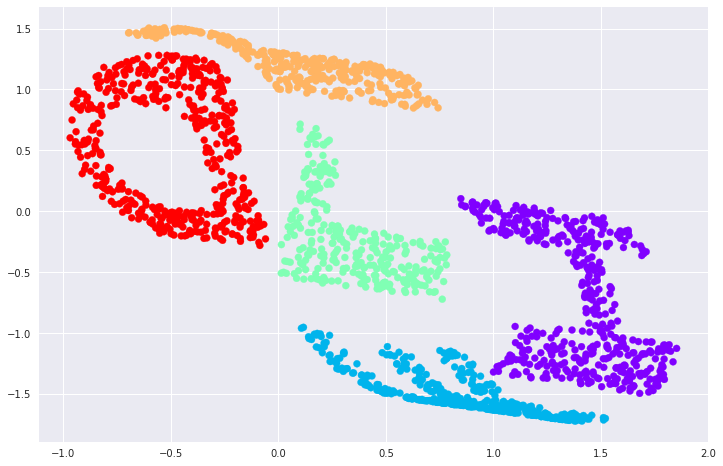
\includegraphics[scale = 0.32]{random_projection_part2.png}
\caption{\label{fig:random_projection_part2}Random Projection applied to curved hello (figure 8) set to reduce it to two dimensions}
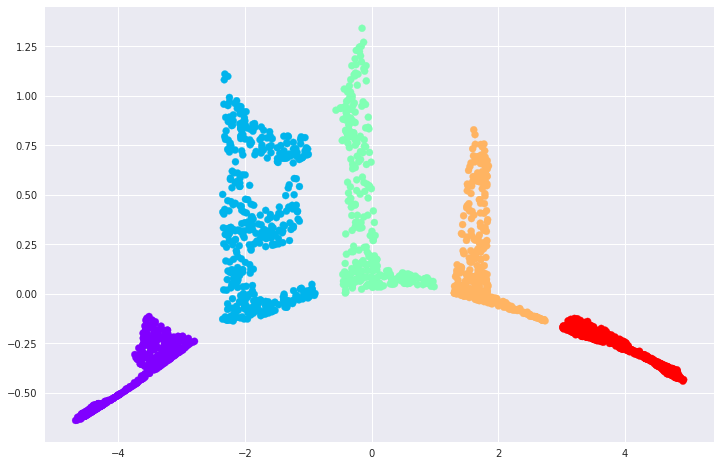
\includegraphics[scale = 0.32]{isomap_part2.png}
\caption{\label{fig:isomap_part2}Isomap applied to curved hello (figure 8) set to reduce it to two dimensions}

\end{figure}

% \begin{figure}[H]
% \centering
% \end{figure}

\begin{figure}[H]
\centering
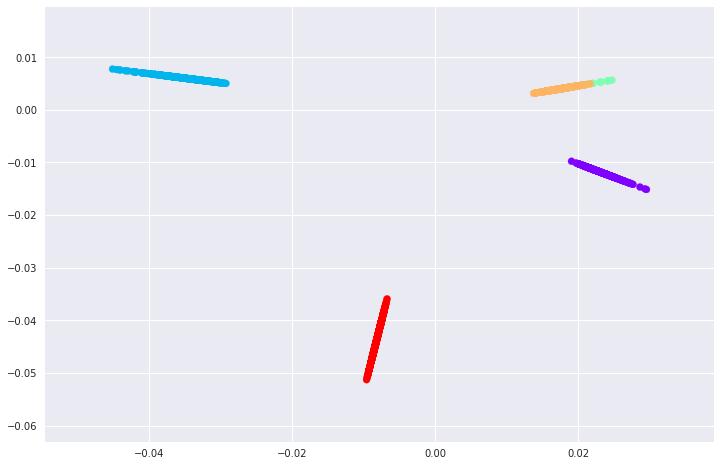
\includegraphics[scale = 0.32]{laplacian_part2.png}
\caption{\label{fig:laplacian_part2}Laplacian applied to curved hello(figure 8) set to reduce it to two dimensions}
\end{figure}

\subsection{Part3}
In the last part, we use a S-shaped data which is curved again. we repeat previous section with this new data.
\begin{figure}[H]
\centering
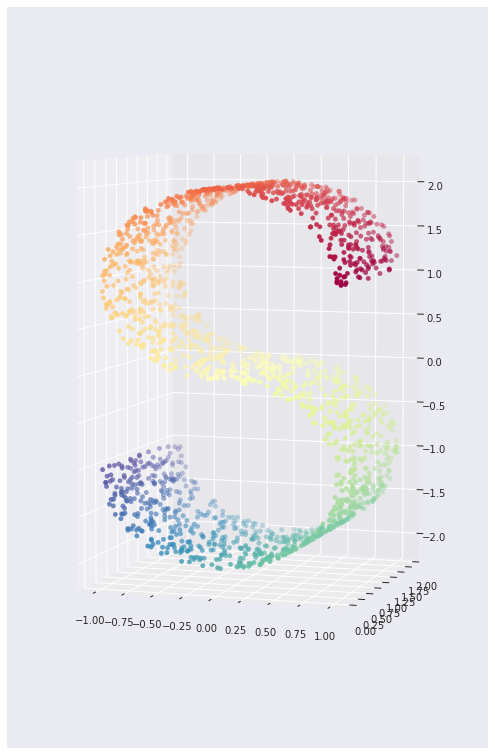
\includegraphics[scale = 0.32]{s_3d.png}
\caption{\label{fig:s_3d}S-shaped curve}
\end{figure}
\newpage
See the result of the the algorithms below:
\begin{figure}[H]
\centering
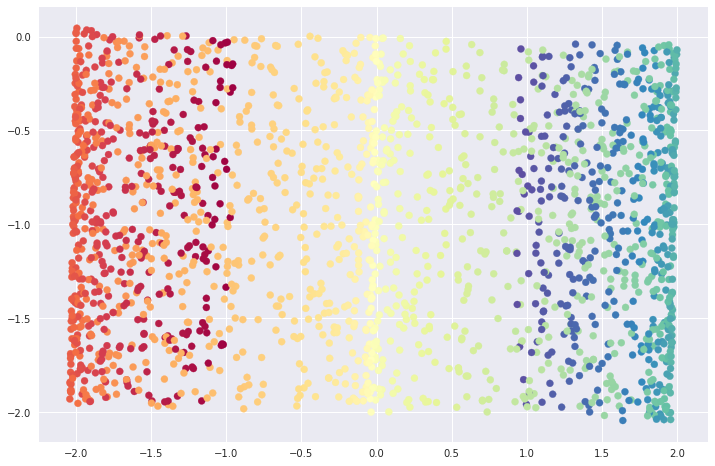
\includegraphics[scale = 0.32]{pca_part3.png}
\caption{\label{fig:pca_part3}PCA applied to S-shaped (figure 13) set to reduce it to two dimensions}
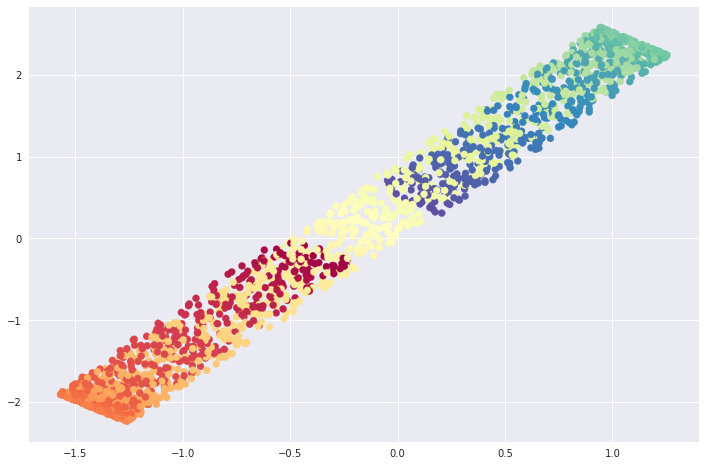
\includegraphics[scale = 0.32]{random_projection_part3.png}
\caption{\label{fig:random_projection_part3}Random Projection applied to S-shaped (figure 13) set to reduce it to two dimensions}

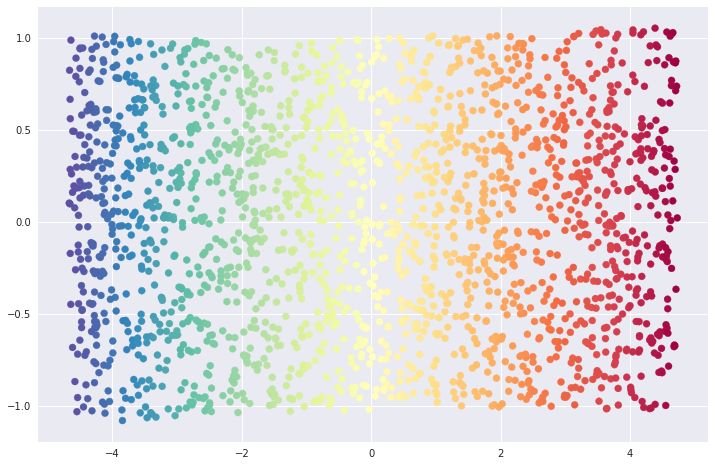
\includegraphics[scale = 0.32]{isomap_part3.png}
\caption{\label{fig:isomap_part3}Isomap applied to S-shaped (figure 13) set to reduce it to two dimensions}
\end{figure}

\begin{figure}[H]

\centering
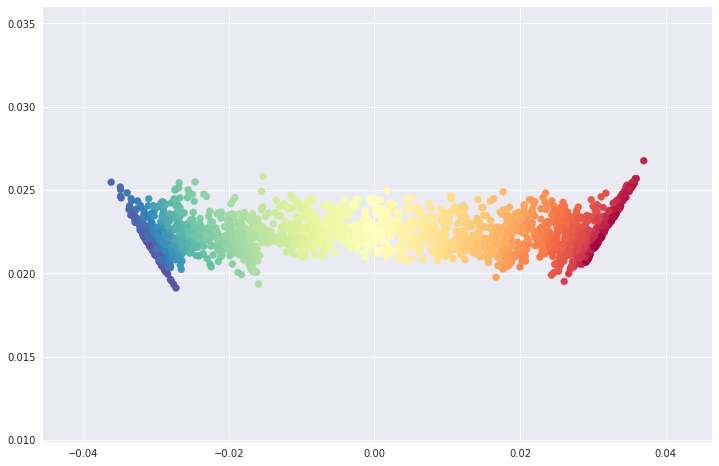
\includegraphics[scale = 0.32]{laplacian_part3.png}
\caption{\label{fig:laplacian_part3}Laplacian applied to S-shaped  (figure 13) set to reduce it to two dimensions}
\end{figure}


% \section{Results and interpretation 2-3 pages}



% \section{Discussion 1/2-1 page}
% Discuss your results. Compare the two values of $n_{s}$ that you've found in the previous section. Compare your results with literature and comment on the difference. If you didn't know the value of the resistance quantum, would you be able to deduce it from your measurements? If yes/no, why?

\newpage
\cite{Kokiopoulou2011}
\cite{Ghodsi2006}
\cite{Projections}
\bibliographystyle{plain}
\bibliography{Mendeley}
\end{document}
